\documentclass[12pt]{article}
\usepackage{array}
\usepackage{amsmath}
\usepackage{amssymb}
\usepackage{algorithm}
\usepackage{algorithmic}
\usepackage{caption}
\usepackage{fontspec}
\usepackage{graphicx}
\usepackage{indentfirst}
\usepackage{minted}
\usepackage{mathtools}
\usepackage{pifont}
\usepackage{setspace}
\usepackage{subfigure}
\usepackage{tikz}
\usepackage{url}
\usepackage{xcolor}
\usepackage{xeCJK}

\usepackage[colorlinks=true]{hyperref}
\usepackage[margin=0.55in]{geometry}

% background color for minted
\definecolor{bg}{rgb}{0.95,0.95,0.95}

% CJK font
\setCJKmainfont{Source Han Serif CN}

% indent value
\setlength{\parindent}{2em}

% line spacing
\linespread{1.2}

% C++ styled text
\newcommand{\CC}{C\nolinebreak\hspace{-.05em}\raisebox{.4ex}{\tiny\bf +}%
\nolinebreak\hspace{-.10em}\raisebox{.4ex}{\tiny\bf +}}

\renewcommand{\thesection}{\Roman{section}}
\renewcommand{\thesubsection}{\thesection-\arabic{subsection}}

\title{简记Ray Tracing in One Weekend}
\author{Yiteng Zhang}

\begin{document}
\maketitle

\noindent{}\textbf{注:}Peter Shirley的\textit{Ray Tracing in One Weekend}系列对入门学习来说特别友好,在写下这篇
记录的时间点,这个系列已经非常有名了。之前有幸读过比较早期的1.X版本,最近听闻该系列的小书推出了一个较大的更新版本,
不免十分好奇,想要看一看新版本的内容变更。另一方面,确实也想再回顾一下这本有趣的小书,所以又一次找出它的最新
版本来看(写这篇简记时,版本为3.2.3)。总体来看,新版本变化还是比较大的,修正了旧版本的一些有误之处,也开始使用
一些modern {\CC}\,特性对之前的实现进行重构(尽管这是作者想要尽量避免的)。无论怎样,这本书是值得再读一读的。回到主题,这篇
简记并非作为其翻译(也不太想那样做),实际上译文很容易获得,已经有不少人完成了转译这项有意义的工作。这篇简记也没有特别
明确的目的,而更像是在阅读时随手记一记的感觉,希望能提炼出点东西。本文应该也不会涉及具体实现,因为书中详细地给出了所有
实现细节,没有任何模糊之处,而且在这里再贴一遍代码也不会对行文与陈述有特别的好处。想来简记的作用也只能是尽量从书中的大量代码
片段中对其所要讲述的技术和原理进行整理,而不必在每次回看时频繁陷入实现细节之中,方便更好地把握书中所涉及的原理和技术的脉络。

\indent{}显然,\textit{Ray Tracing in One Weekend}这本书是讲渲染的。具体来说,是讲述有关如何从零开始构建
一个光线追踪渲染器(即Raytracer)的书。这本书不打算讨论渲染领域中涉及到的艰深部分,而是以体验式的方
式,手把手地带领我们领略光线追踪渲染的美妙所在。尽管不打算实现一个功能完备的渲染器,其讲述方式却并不随便,反而可以说是
比较严谨的,不会让人感觉学不到真东西。

\indent{}想要渲染图像,那我们最后肯定是要得到能够真真切切看得到的结果。常见的图像格式都有自己的编解码过程,想要
不借助第三方库而得到对应的图像格式,其实是比较困难的。当然了,一些比较常用的header-only库如\texttt{stb\_image}可以帮我们
做这件事,但毕竟还是有一些额外工作要做。针对这个问题,书中推荐使用PPM格式,简单查一下就可以发现它是直接存文本的,只要能
找到合适的PPM解析器,就可以直接看到渲染出来的图像了,可以让我们暂时不必考虑出图编码的问题。

\indent{}渲染基础涉及到的操作基本上就是一点线性代数的内容,所以首先需要写代码来处理向量,实现一些辅助函数,大体上
是点积、叉积、向量单位化,还有求向量长度这些基本操作。具体的实现书里给出了一个,我们也可以自己写。无论如何,实现
这些操作总归是挺简单的事情,真正需要考虑的要点是约定何种输入输出形式,以方便后续使用。

\indent{}一旦完成了上面的准备工作,就可以开始考虑如何绘制我们的三维场景。第一个问题是,ray是怎样的东西?
Ray tracing意为光线追踪,而这里的ray实际上也是符合射线(ray)的几何定义的。我们从一个端点$\bf{A}$出发,沿着某个方向
$\bf{b}$发出一条射线(或者说光线),其描述应该是:
\begin{equation}
\mathbf{P}(t) = \mathbf{A} + t\mathbf{b},\; t\in\mathbb{R}
\end{equation}
\noindent{}注意到$t$可以是负的,也就是说沿着与方向$\bf{b}$相反的方向投射。

\indent{}我们清楚光线追踪的核心原理:从相机中心朝着screen上的每个像素发出ray,这些ray与场景中的物体相交,通过计算
交点处的颜色来得到对应像素的颜色。现在我们已经清楚ray的表达,是时候对相机进行建模了,先来看一个简单的例子:
\begin{figure}[h]
\centering
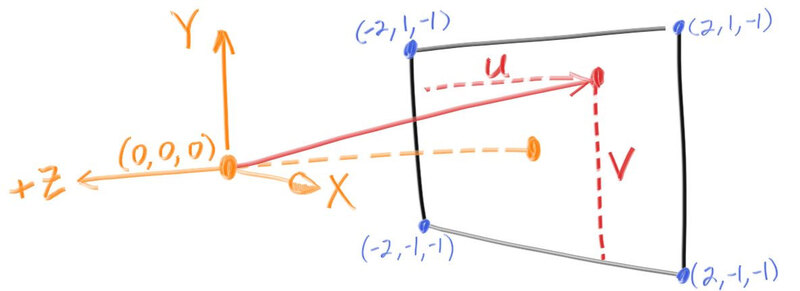
\includegraphics[width=0.65\textwidth]{./imgs/fig-1.03-cam-geom.jpg}
\end{figure}

\indent{}可以看到该相机直接被放在世界坐标系的原点,因而对应的相机坐标系的原点与世界坐标系的原点是重合的。另外,该相机的三个轴也
是与世界坐标系的坐标轴align的,可以说是相当特殊而又简单的一个例子,这便于我们进行渲染器的初期构建。同时,注意到相机中心到
投影平面的距离被设置为单位距离,这也是一项简化,可以说我们的virtual camera的焦距是单位值。

\end{document}